\documentclass[12pt, letterpaper]{article}
\usepackage[margin=0.5in]{geometry}
\usepackage{amsmath}
\usepackage{amssymb}
\usepackage{fancyvrb}
\usepackage{graphicx}
\graphicspath{ {./images/} }

\title{Q2 Assignment 2 Report}
\author{Lokesh Mohanty (SR no: 21014)}
\date{November 2022}

\begin{document}

\maketitle

\section{Computer \& Compiler Details}
\label{sec:comp}

\subsection{Basic Information}
\label{sec:basic}
\begin{tabular}{ll}
  Architecture    &: x86\_64\\
  CPU op-mode(s)  &: 32-bit, 64-bit\\
  Address sizes   &: 48 bits physical, 48 bits virtual\\
  Byte Order      &: Little Endian\\
  CPU(s)          &: 16\\
\end{tabular}

\subsection{CPU Details}
\label{sec:cpu}
\begin{tabular}{ll}
  Vendor ID       &: AuthenticAMD\\
  Model name            &: AMD Ryzen 7 PRO 5875U with Radeon Graphics\\
  CPU family            &: 25\\
  Model                 &: 80\\
  Thread(s) per core    &: 2\\
  Core(s) per socket    &: 8\\
  Socket(s)             &: 1\\
  Stepping              &: 0\\
  Frequency boost       &: enabled\\
  CPU(s) scaling MHz    &: 44\%\\
  CPU max MHz           &: 4546.8750\\
  CPU min MHz           &: 1600.0000\\
\end{tabular}

\subsection{Cache}
\label{sec:cache}
\begin{tabular}{ll}
  L1d cache  &: 256 KiB (8 instances)\\
  L1i cache  &: 256 KiB (8 instances)\\
  L2 cache   &: 4 MiB (8 instances)\\
  L3 cache   &: 16 MiB (1 instance)\\
\end{tabular}

\subsection{Compiler Details}
\label{sec:compiler}

\begin{tabular}{ll}
  Compiler &: gcc (GCC)\\
  Version  &: 10.2.1 20201203\\
\end{tabular}

\section{Results}
\label{sec:results}

I tested with the 3 samples of data given and plotted the time taken for matrix vector multiplication with 1, 2, 4 and 8 threads.

\textbf{Time Taken:}\\

\begin{tabular}{ |c|c|c|c|c| }
 \hline
 Test Case &Number of Threads &N\_1e2 &N\_1e3 &N\_1e4 \\
 \hline
 1         &1      &0.312ms     &3.146ms         &278ms        \\
 2         &2      &0.167ms     &2.056ms         &144ms        \\
 3         &4      &0.141ms     &1.693ms         &77ms        \\
 4         &8      &0.183ms     &1.044ms        &54ms        \\
 \hline
\end{tabular}

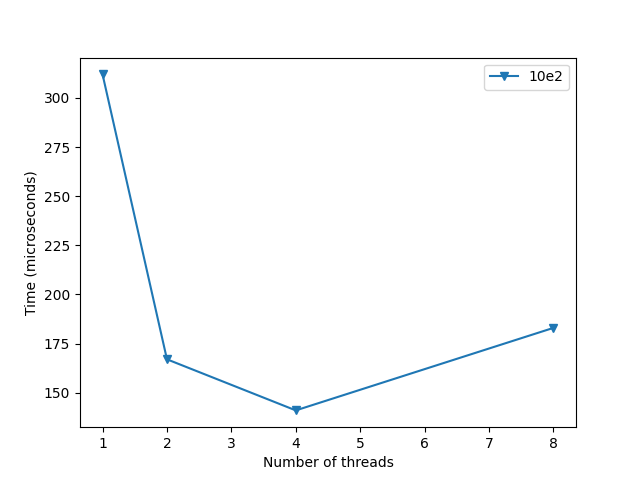
\includegraphics{3}

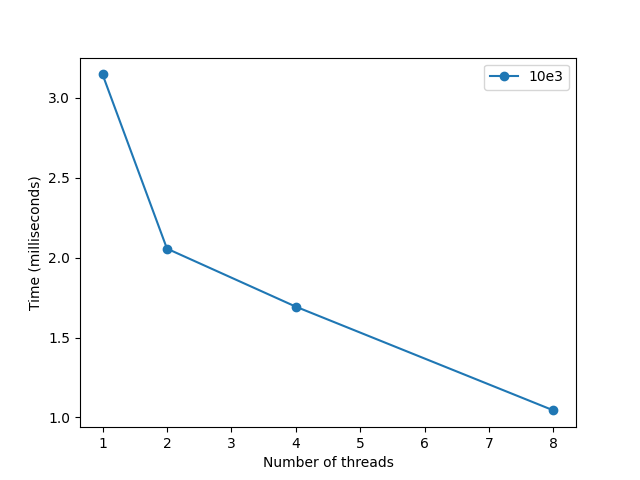
\includegraphics{2}

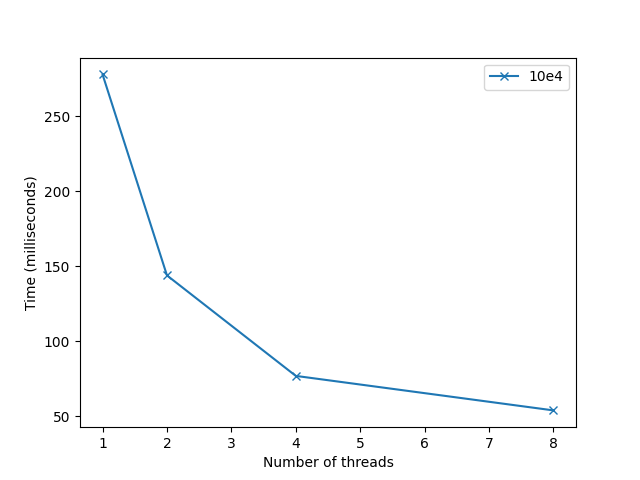
\includegraphics{1}

\subsection{Analysis}
\label{sec:analysis}

We can see that as we increase the number of thereads, the time taken decreases. But the decrease is not linear as the whole program is not parallelizable.\\

We also see that in case of low input data the time increases with increase in number of threads after crossing a thresold. This happens due to the information passing time being more than the speedup obtained.



\end{document}


%%% Local Variables:
%%% mode: latex
%%% TeX-master: t
%%% End:
